\documentclass[a4paper,titlepage]{article}
\usepackage[utf8]{inputenc}
\usepackage{fullpage}
\usepackage{indentfirst}
\usepackage[per-mode=symbol]{siunitx}
\usepackage{listings}
\usepackage{graphicx}
\usepackage{color}
\usepackage{amsmath}
\usepackage{array}
\usepackage[hidelinks]{hyperref}
\usepackage[format=plain,font=it]{caption}
\usepackage{subcaption}
\usepackage{standalone}
\usepackage[nottoc]{tocbibind}
\usepackage{cleveref}
\usepackage{listings}
\usepackage{titlesec}
\usepackage{minted}
\usepackage{booktabs}
\usepackage{csvsimple}
\usepackage{siunitx}
\usepackage[super]{nth}

% Custom commands
\newcommand\numberthis{\addtocounter{equation}{1}\tag{\theequation}}
\newcommand{\code}[1]{\texttt{#1}}
\newcolumntype{P}[1]{>{\centering\arraybackslash}p{#1}}

\setminted{linenos,breaklines,fontsize=\footnotesize}

%\titleformat*{\section}{\normalsize\bfseries}
%\titleformat*{\subsection}{\small\bfseries}
\renewcommand{\thesubsection}{\thesection.\alph{subsection}}
\providecommand*{\listingautorefname}{Listing}

%opening
\title{\textbf{ECSE 543 \\ Assignment 1}}
\author{Sean Stappas \\ 260639512}
\date{October \nth{17}, 2017}

\begin{document}
	\sloppy
	\maketitle
	\twocolumn
	
	\section{Introduction}
	
	The programs for this assignment were created in Python 2.7. The source code is provided as listings in \autoref{appendix:listings}. To perform the required tasks in this assignment, a custom matrix package was created, with useful methods such as add, multiply, transpose, etc. This package can be seen in \autoref{lst:matrices}. In addition, logs of the output of the programs are provided in \autoref{appendix:logs}.
	
	\section{Choleski Decomposition}
	
	The source code for the Question 1 main program can be seen in \autoref{lst:q1}.
	
	\subsection{Choleski Program}
	% Write a program to solve the matrix equation Ax=b by Choleski decomposition. A is a real, symmetric, positive-definite matrix of order n.
	
	The code relating specifically to Choleski decomposition can be seen in \autoref{lst:choleski}.
	
	
	\subsection{Constructing Test Matrices}
	% Construct some small matrices (n = 2, 3, 4, or 5) to test the program. Remember that the matrices must be real, symmetric and positive-definite. Explain how you chose the matrices.
	
	The matrices were constructed with the knowledge that, if $A$ is positive-definite, then $A = LL^T$ where L is a lower triangular non-singular matrix. The task of choosing valid $A$ matrices then boils down to finding non-singular lower triangular $L$ matrices. To ensure that $L$ is non-singular, one must simply choose nonzero values for the main diagonal.
	
	\subsection{Test Runs}
	% Test the program you wrote in (a) with each small matrix you built in (b) in the following way: invent an x, multiply it by A to get b, then give A and b to your program and check that it returns x correctly.
	
	The matrices were tested by inventing $x$ matrices, and checking that the program solves for that $x$ correctly. The output of the program, comparing expected and obtained values of $x$, can be seen in \autoref{lst:q1_log}.
	
	\subsection{Linear Networks}
	% Write a program that reads from a file a list of network branches (Jk, Rk, Ek) and a reduced incidence matrix, and finds the voltages at the nodes of the network. Use the code from part (a) to solve the matrix problem. Explain how the data is organized and read from the file. Test the program with a few small networks that you can check by hand. Compare the results for your test circuits with the analytical results you obtained by hand. Cleary specify each of the test circuits used with a labeled schematic diagram.
	
	First, the program was tested on the circuits provided on MyCourses.
	
	% TODO: Put pictures of test circuits! (create your own as well as the provided ones…)
	
	\section{Finite Difference Mesh}
	
	The source code for the Question 2 main program can be seen in \autoref{lst:q2}.
	
	\subsection{Equivalent Resistance}
	% Using the program you developed in question 1, find the resistance, R, between the node at the bottom left corner of the mesh and the node at the top right corner of the mesh, for N = 2, 3, …, 10. (You will probably want to write a small program that generates the input file needed by the network analysis program. Constructing by hand the incidence matrix for a 200-node network is rather tedious).
	
	The code for creating all the network matrices and for finding the equivalent resistance of an $N$ by $2N$ mesh can be seen in \autoref{lst:linear_networks}. The resistances found by the program for values of $N$ from 2 to 10 can be seen in \autoref{table:q2a}.
	
	\begin{table}[!htb]
		\centering
		\caption{Mesh equivalent resistance R versus mesh size N.}
		\csvautobooktabular{csv/q2a.csv}
		\label{table:q2a}
	\end{table}

	The resistance values returned by the program for small meshes were validated using simple SPICE circuits. % TODO: Show SPICE figure...
	
	\subsection{Time Complexity}
	% In theory, how does the computer time taken to solve this problem increase with N, for large N? Are the timings you observe for your practical implementation consistent with this? Explain your observations.
	
	The runtime data for the mesh resistance solver is tabulated in \autoref{table:q2b} and plotted in \autoref{fig:q2b}. Theoretically, the time complexity of the program should be $O(N^6)$, and this matches the obtained data.
	
	\begin{table}[!htb]
		\centering
		\caption{Runtime of mesh resistance solver program versus mesh size $N$.}
		\csvautobooktabular{csv/q2b.csv}
		\label{table:q2b}
	\end{table}

	\begin{figure}[!htb]
		\centering
		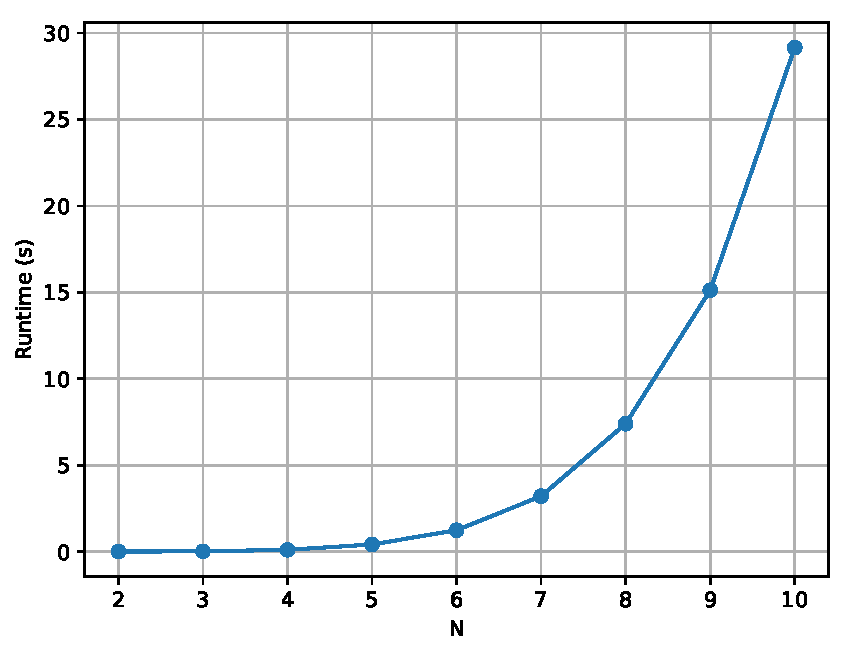
\includegraphics[width=\columnwidth]{plots/q2b.pdf}
		\caption
		{Runtime of mesh resistance solver program versus mesh size $N$.}
		\label{fig:q2b}
	\end{figure}
	
	\subsection{Sparsity Modification}
	% Modify your program to exploit the sparse nature of the matrices to save computation time. What is the half-bandwidth b of your matrices? In theory, how does the computer time taken to solve this problem increase now with N, for large N? Are the timings you for your practical sparse implementation consistent with this? Explain your observations.
	
	The runtime data for the banded mesh resistance solver is tabulated in \autoref{table:q2c} and plotted in \autoref{fig:q2c}. By inspection of the constructed network matrices, a half-bandwidth of $2N + 1$ was chosen. Theoretically, the banded version should have a time complexity of $O(N^4)$.
	
	\begin{table}[!htb]
		\centering
		\caption{Runtime of banded mesh resistance solver program versus mesh size $N$.}
		\csvautobooktabular{csv/q2c.csv}
		\label{table:q2c}
	\end{table}

	\begin{figure}[!htb]
		\centering
		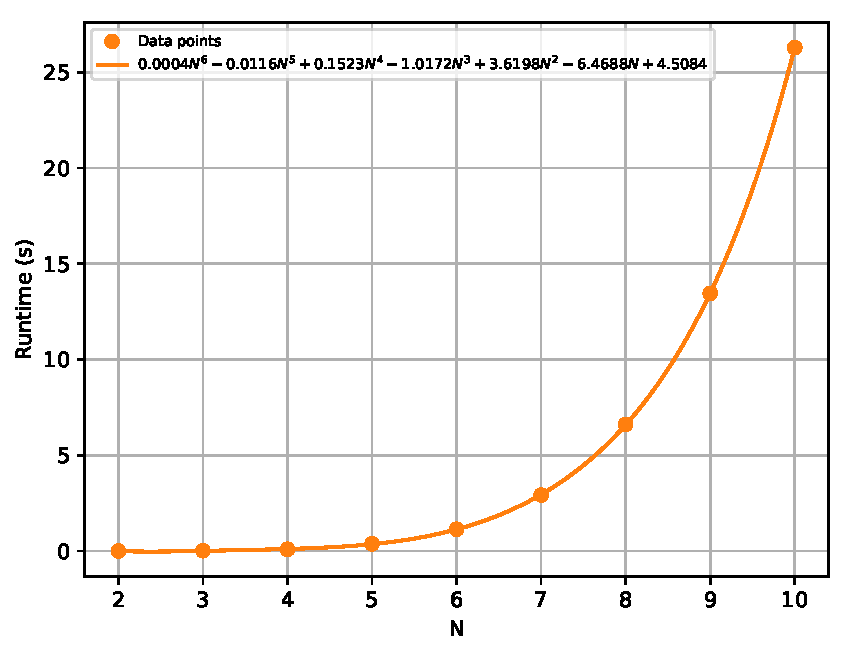
\includegraphics[width=\columnwidth]{plots/q2c.pdf}
		\caption
		{Runtime of banded mesh resistance solver program versus mesh size $N$.}
		\label{fig:q2c}
	\end{figure}

	% TODO: Fix banded method (complexity doesn't make sense...)

	The runtime of the banded and non-banded versions of the program are plotted in \autoref{fig:q2bc}, showing the benefits of banded elimination.

	\begin{figure}[!htb]
		\centering
		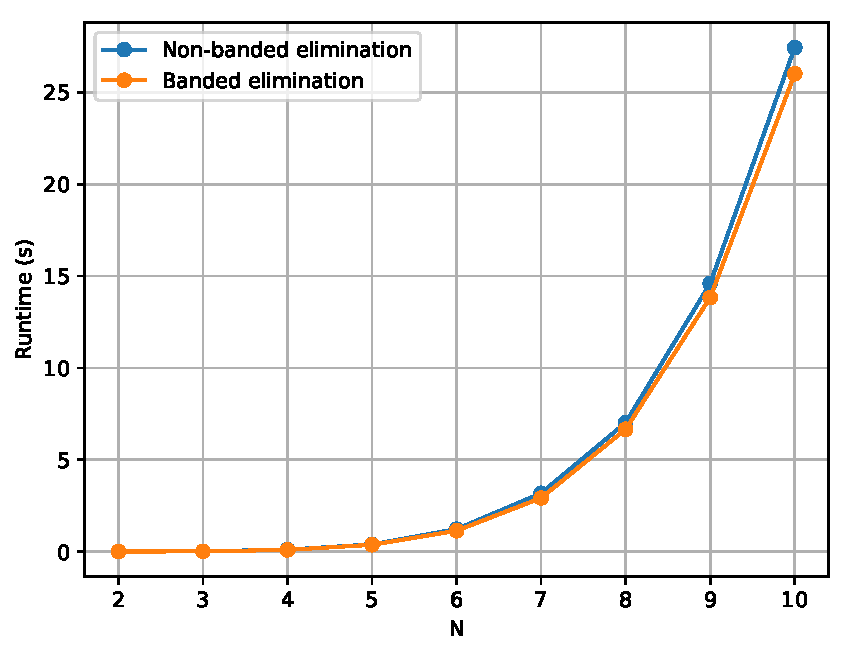
\includegraphics[width=\columnwidth]{plots/q2bc.pdf}
		\caption
		{Comparison of runtime of banded and non-banded resistance solver programs versus mesh size $N$.}
		\label{fig:q2bc}
	\end{figure}
	
	\subsection{Resistance vs. Mesh Size}
	% Plot a graph of R versus N. Find a function R(N) that fits the curve reasonably well and is asymptotically correct as N tends to infinity, as far as you can tell.
	
	The equivalent mesh resistance $R$ is plotted versus the mesh size $N$ in \autoref{fig:q2d}. The function $R(N)$ appears logarithmic, and a log function does indeed fit the data well.
	
	\begin{figure}[!htb]
		\centering
		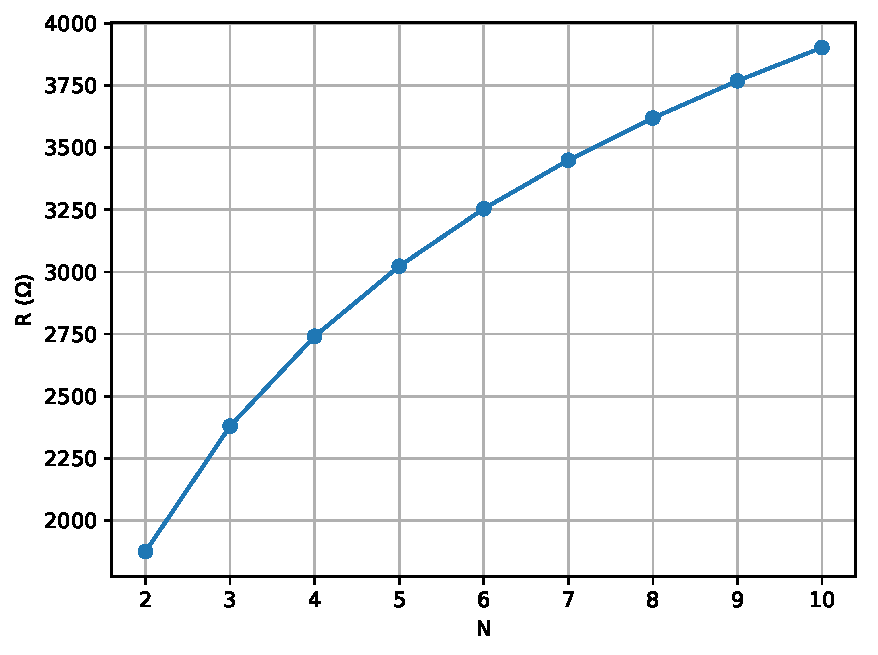
\includegraphics[width=\columnwidth]{plots/q2d.pdf}
		\caption
		{Resistance of mesh versus mesh size $N$.}
		\label{fig:q2d}
	\end{figure}
	
	\section{Coaxial Cable}
	
	The source code for the Question 2 main program can be seen in \autoref{lst:q3}.
	
	\subsection{SOR Program}
	% Write a computer program to find the potential at the nodes of a regular mesh in the air between the conductors by the method of finite differences. Use a five-point difference formula. Exploit at least one of the planes of mirror symmetry that this problem has. Use an	equal node-spacing, h, in the x and y directions. Solve the matrix equation by successive	over-relaxation (SOR), with SOR parameter w. Terminate the iteration when the magnitude	of the residual at each free node is less than 10^-5.
	
	The source code for the finite difference methods can be seen in \autoref{lst:finite_diff}. Horizontal and vertical symmetries were exploited by only solving for a quarter of the coaxial cable, and reproducing the results where necessary.
	
	\subsection{Varying $\omega$}
	% With h = 0.02, explore the effect of varying w. For 10 values of w between 1.0 and 2.0,	tabulate the number of iterations taken to achieve convergence, and the corresponding value	of potential at the point (x ,y) = (0.06, 0.04). Plot a graph of number of iterations versus w.
	
	The number of iterations to achieve convergence for 10 values of $\omega$ between 1 and 2 are tabulated in \autoref{table:q3b_iterations} and plotted in \autoref{fig:q3b}. Based on these results, the value of $\omega$ yielding the minimum number of iterations is 1.3.
	
	\begin{table}[!htb]
		\centering
		\caption{Number of iterations of SOR versus $\omega$.}
		\csvautobooktabular{csv/q3b_iterations.csv}
		\label{table:q3b_iterations}
	\end{table}
	
	\begin{figure}[!htb]
		\centering
		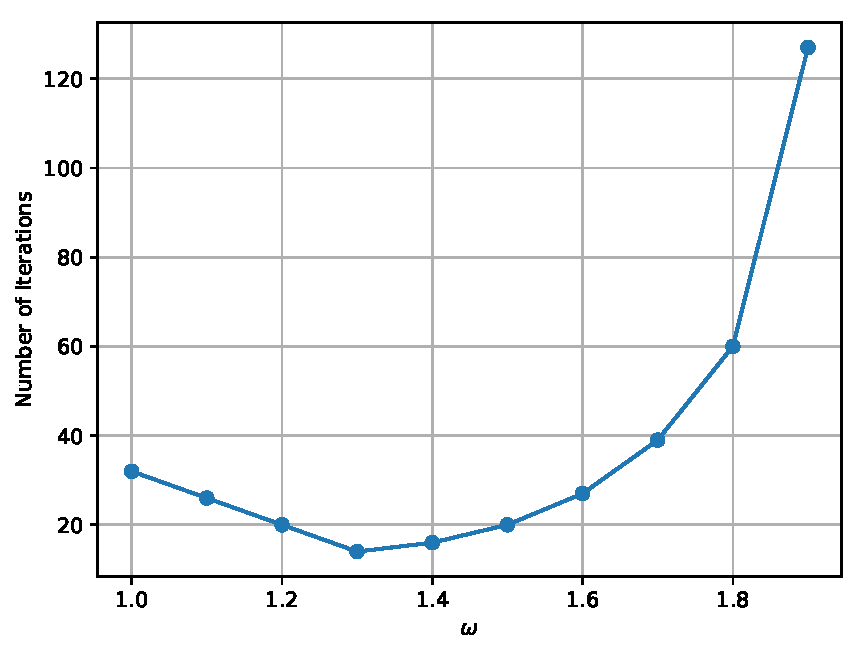
\includegraphics[width=\columnwidth]{plots/q3b.pdf}
		\caption
		{Number of iterations of SOR versus $\omega$.}
		\label{fig:q3b}
	\end{figure}

	The potential values found at (0.06, 0.04) versus $\omega$ are tabulated in \autoref{table:q3b_potential}. It can be seen that all the potential values are identical to 3 decimal places.

	\begin{table}[!htb]
		\centering
		\caption{Potential at (0.06, 0.04) versus $\omega$ when using SOR.}
		\csvautobooktabular{csv/q3b_potential.csv}
		\label{table:q3b_potential}
	\end{table}
	
	\subsection{Varying $h$}
	% With an appropriate value of w, chosen from the above experiment, explore the effect of	decreasing h on the potential. Use values of h = 0.02, 0.01, 0.005, etc, and both tabulate and	plot the corresponding values of potential at (x, y) = (0.06, 0.04) versus 1/h. What do you think is the potential at (0.06, 0.04), to three significant figures? Also, tabulate and plot the number of iterations versus 1/h. Comment on the properties of both plots.
	
	With $\omega = 1.3$, the number of iterations of SOR versus $1/h$ is tabulated in \autoref{table:q3c_iterations} and plotted in \autoref{fig:q3c_iterations}. It can be seen that the smaller the node spacing is, the more iterations the program will take to run. Theoretically, the time complexity of the program should be $O(N^3)$, where the finite difference mesh is $N$ by $N$, and this matches the measured data.
	
	\begin{table}[!htb]
		\centering
		\caption{Number of iterations of SOR versus $1/h$. Note that $\omega=1.3$.}
		\csvautobooktabular{csv/q3c_iterations.csv}
		\label{table:q3c_iterations}
	\end{table}
	
	\begin{figure}[!htb]
		\centering
		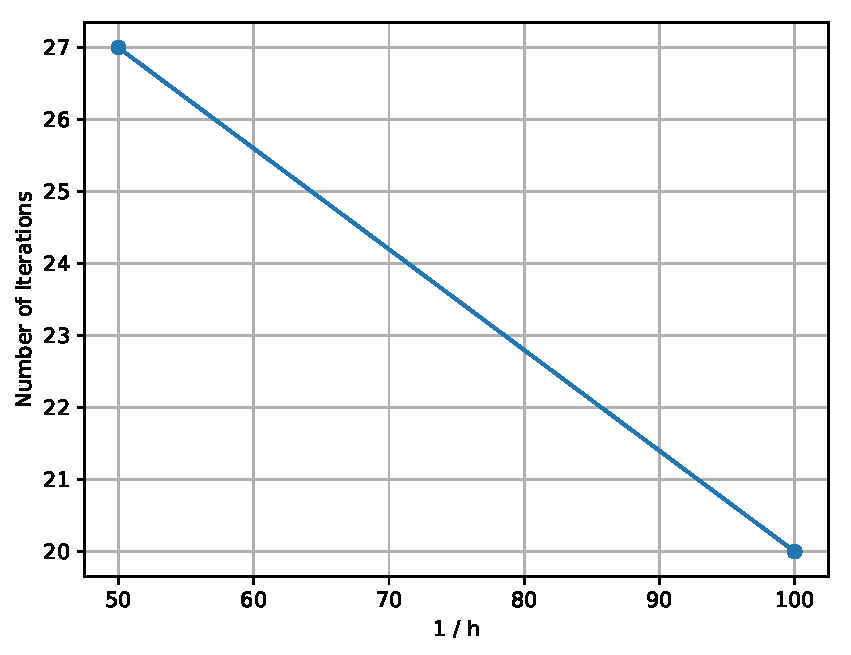
\includegraphics[width=\columnwidth]{plots/q3c_iterations.pdf}
		\caption
		{Number of iterations of SOR versus $1/h$. Note that $\omega=1.3$.}
		\label{fig:q3c_iterations}
	\end{figure}

	The potential values found at (0.06, 0.04) versus $1/h$ are tabulated in \autoref{table:q3c_potential} and plotted in \autoref{fig:q3c_potential}. By examining these values, the potential at (0.06, 0.04) to three significant figures is approximately \SI{5.25}{\volt}. It can be seen that the smaller the node spacing is, the more accurate the calculated potential is. However, by inspecting \autoref{fig:q3c_potential} it is apparent that the potential converges relatively quickly to around \SI{5.25}{\volt} There are therefore diminishing returns to decreasing the node spacing too much, since this will also increase the runtime of the program.

	\begin{table}[!htb]
		\centering
		\caption{Potential at (0.06, 0.04) versus $1/h$ when using SOR.}
		\csvautobooktabular{csv/q3c_potential.csv}
		\label{table:q3c_potential}
	\end{table}

	\begin{figure}[!htb]
		\centering
		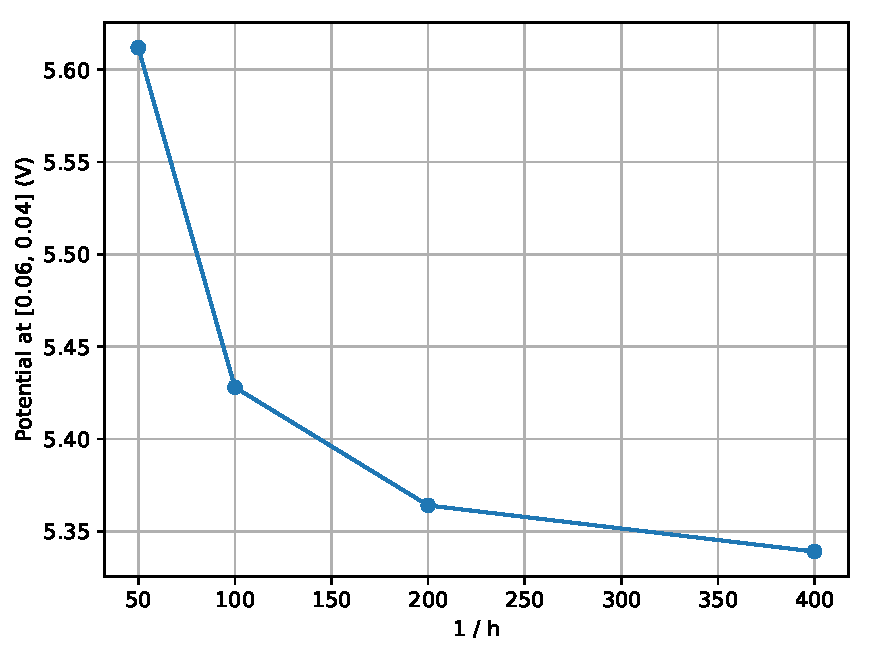
\includegraphics[width=\columnwidth]{plots/q3c_potential.pdf}
		\caption
		{Potential at (0.06, 0.04) found by SOR versus $1/h$. Note that $\omega=1.3$.}
		\label{fig:q3c_potential}
	\end{figure}
	
	\subsection{Jacobi Method}
	% Use the Jacobi method to solve this problem for the same values of h used in part (c). Tabulate and plot the values of the potential at (x, y) = (0.06, 0.04) versus 1/h and the number of iterations versus 1/h. Comment on the properties of both plots and compare to those of SOR.
	
	The number of iterations of the Jacobi method versus $1/h$ is tabulated in \autoref{table:q3d_iterations} and plotted in \autoref{fig:q3d_iterations}. Similarly to SOR, the smaller the node spacing is, the more iterations the program will take to run. We can see however that the Jacobi method takes a much larger number of iterations to converge. Theoretically, the Jacobi method should have a time complexity of $O(N^4)$, and this matches the data.
	
	\begin{table}[!htb]
		\centering
		\caption{Number of iterations versus $\omega$ when using the Jacobi method.}
		\csvautobooktabular{csv/q3d_iterations.csv}
		\label{table:q3d_iterations}
	\end{table}

	\begin{figure}[!htb]
		\centering
		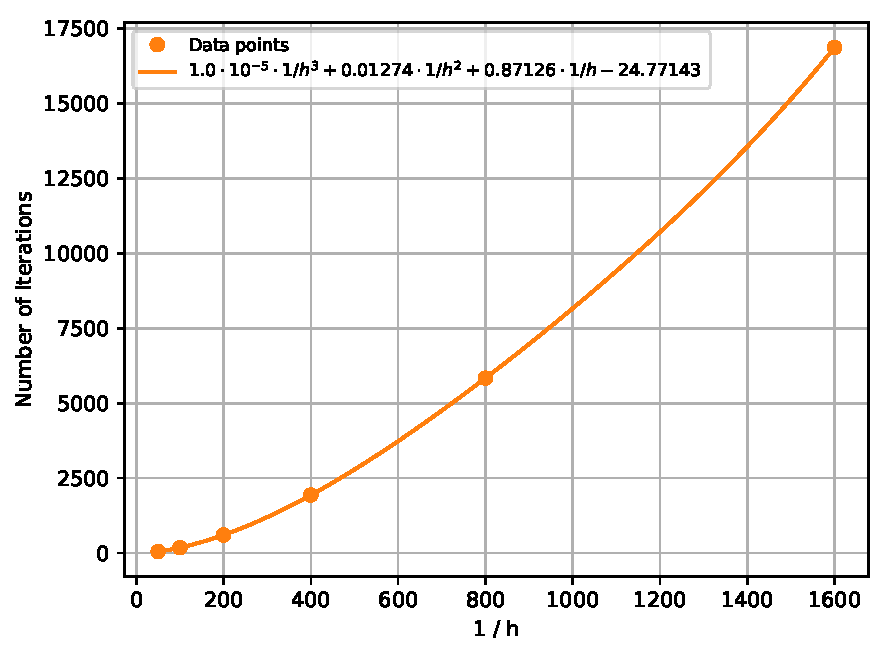
\includegraphics[width=\columnwidth]{plots/q3d_iterations.pdf}
		\caption
		{Number of iterations of the Jacobi method versus $1/h$.}
		\label{fig:q3d_iterations}
	\end{figure}

	The potential values found at (0.06, 0.04) versus $1/h$ with the Jacobi method are tabulated in \autoref{table:q3d_potential} and plotted in \autoref{fig:q3d_potential}. These potential values are almost identical to the SOR ones. Similarly to SOR, the smaller the node spacing is, the more accurate the calculated potential is.

	\begin{table}[!htb]
		\centering
		\caption{Potential at (0.06, 0.04) versus $1/h$ when using the Jacobi method.}
		\csvautobooktabular{csv/q3d_potential.csv}
		\label{table:q3d_potential}
	\end{table}

	\begin{figure}[!htb]
		\centering
		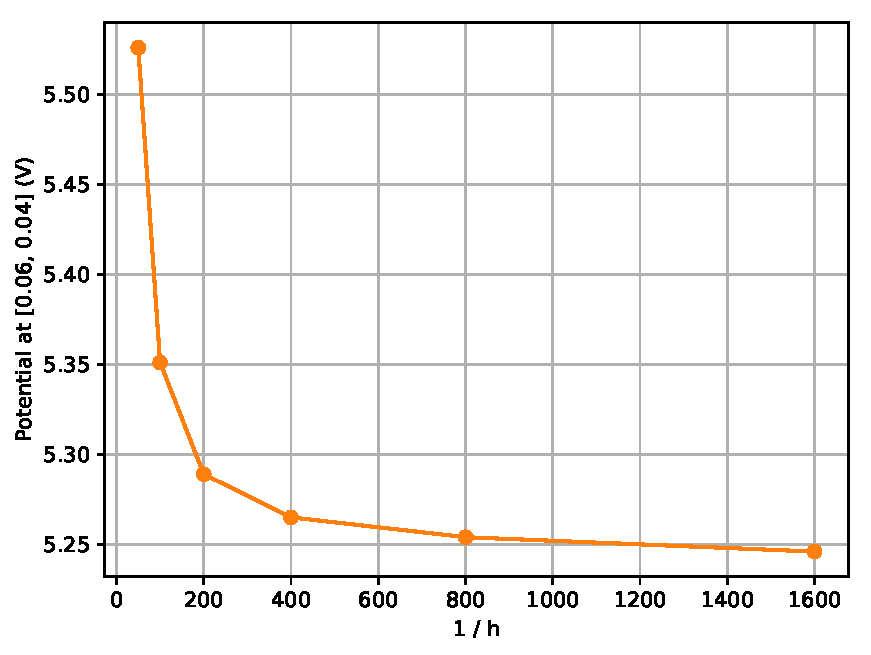
\includegraphics[width=\columnwidth]{plots/q3d_potential.pdf}
		\caption
		{Potential at (0.06, 0.04) versus $1/h$ when using the Jacobi method.}
		\label{fig:q3d_potential}
	\end{figure}

	The number of iterations of both SOR and the Jacobi method can be seen in \autoref{fig:q3d_iterations_comparison}, which shows the clear benefits of SOR.

	\begin{figure}[!htb]
		\centering
		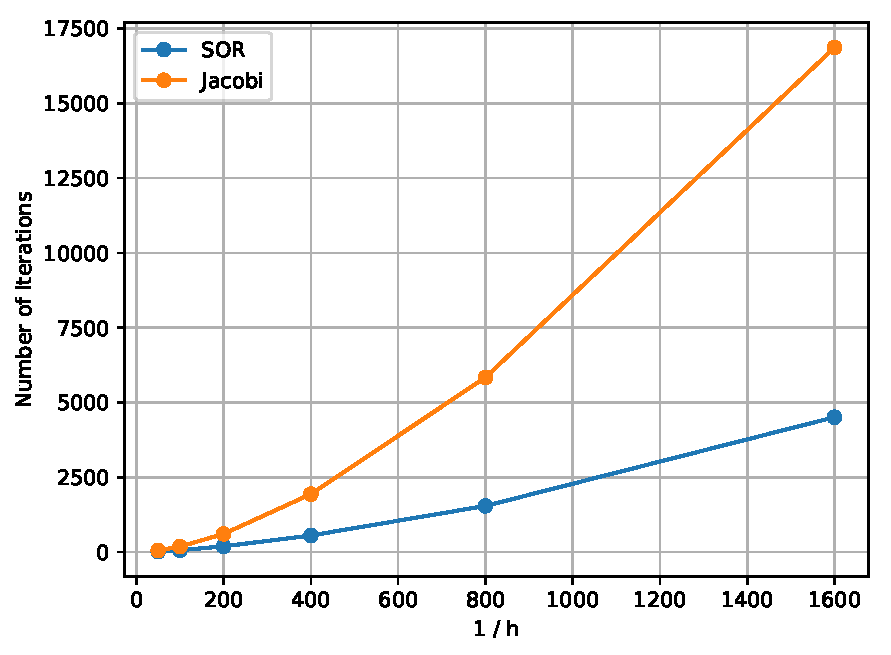
\includegraphics[width=\columnwidth]{plots/q3d_iterations_comparison.pdf}
		\caption
		{Comparison of number of iterations when using SOR and Jacobi methods versus $1/h$. Note that $\omega=1.3$ for the SOR program.}
		\label{fig:q3d_iterations_comparison}
	\end{figure}
	
	\subsection{Non-uniform Node Spacing}
	% Modify the program you wrote in part (a) to use the five-point difference formula derived in	class for non-uniform node spacing. An alternative to using equal node spacing, h, is to use	smaller node spacing in more “difficult” parts of the problem domain. Experiment with a	scheme of this kind and see how accurately you can compute the value of the potential at (x, y)	= (0.06, 0.04) using only as many nodes as for the uniform case h = 0.01 in part (c).
	
	First, we adjust the equation derived in class to set $a_1 = \Delta_x\alpha_1$, $a_2 = \Delta_x\alpha_2$, $b_1 = \Delta_y\beta_1$ and $b_2 = \Delta_y\beta_2$. These values correspond to the distances between adjacent nodes \footnote{Note that, in the program, index $i$ is associated to position $x$ and index $j$ is associated to position $y$. This is purely for easier printing of the matrices.}, and can be easily calculated by the program. Then, the five-point difference formula for non-uniform spacing can be seen in \autoref{eq:non_uniform}.
	
	\begin{align} \label{eq:non_uniform}
		\begin{split}
			\phi^{k + 1}_{i,j} = 
			&\frac{1}{a_1 + a_2}\left(\frac{\phi^k_{i - 1,j}}{a_1} + \frac{\phi^k_{i + 1,j}}{a_2}\right) + \\
			&\frac{1}{b_1 + b_2}\left(\frac{\phi^k_{i, j - 1}}{b_1} + \frac{\phi^k_{i, j + 1}}{b_2}\right)
		\end{split}
	\end{align}
	
	This was implemented in the finite difference program, as seen in \autoref{lst:finite_diff}. As can be seen in this code, many different mesh arrangements were tested. The arrangement that was chosen can be seen in \autoref{fig:q3e}. The potential obtained from this arrangement is \SI{5.083}{\volt}, which seems like a more accurate potential value.
	
	\begin{figure}[!htb]
		\centering
		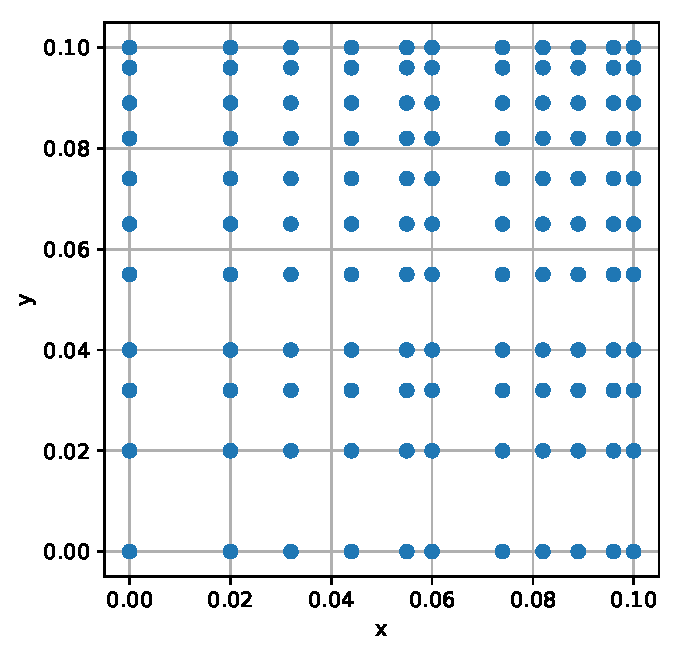
\includegraphics[width=\columnwidth]{plots/q3e.pdf}
		\caption
		{Final mesh arrangement used for non-uniform node spacing. Each point corresponds to a mesh point.}
		\label{fig:q3e}
	\end{figure}
	
	\onecolumn
	
	\appendix
	
	\section{Code Listings} \label{appendix:listings}
	
	\begin{center}
		\captionof{listing}{Custom matrix package (\texttt{matrices.py}).}
		\inputminted{python}{../matrices.py}
		\label{lst:matrices}
	\end{center}

	\begin{center}
		\captionof{listing}{Choleski decomposition (\texttt{choleski.py}).}
		\inputminted{python}{../choleski.py}
		\label{lst:choleski}
	\end{center}

	\begin{center}
		\captionof{listing}{Linear resistive networks (\texttt{linear\_networks.py}).}
		\inputminted{python}{../linear_networks.py}
		\label{lst:linear_networks}
	\end{center}
	
	\begin{center}
		\captionof{listing}{Finite difference method (\texttt{finite\_diff.py}).}
		\inputminted{python}{../finite_diff.py}
		\label{lst:finite_diff}
	\end{center}
	
	\begin{center}
		\captionof{listing}{Question 1 (\texttt{q1.py}).}
		\inputminted{python}{../q1.py}
		\label{lst:q1}
	\end{center}
	
	\begin{center}
		\captionof{listing}{Question 2 (\texttt{q2.py}).}
		\inputminted{python}{../q2.py}
		\label{lst:q2}
	\end{center}

	\begin{center}
		\captionof{listing}{Question 3 (\texttt{q3.py}).}
		\inputminted{python}{../q3.py}
		\label{lst:q3}
	\end{center}

	\section{Output Logs} \label{appendix:logs}
	
	\begin{center}
		\captionof{listing}{Output of Question 1 program (\texttt{q1.txt}).}
		\inputminted{pycon}{logs/q1.txt}
		\label{lst:q1_log}
	\end{center}

	\begin{center}
		\captionof{listing}{Output of Question 2 program (\texttt{q2.txt}).}
		\inputminted{pycon}{logs/q2.txt}
		\label{lst:q2_log}
	\end{center}
	
	\begin{center}
		\captionof{listing}{Output of Question 3 program (\texttt{q3.txt}).}
		\inputminted{pycon}{logs/q3.txt}
		\label{lst:q3_log}
	\end{center}

\end{document}
